\subsection{Software Architecture}
\label{sec:software}

This section presents the open software architecture of the proposed system \footnote{\url{https://github.com/lsa-pucrs/donnie-assistive-robot-sw}}. We adopt a top-down presentation approach, initially presenting a discussion about choosing an appropriate programming language for people with visual disability. Next, we discuss the developed 
%assistive IDE, the 
graphical simulation environment, the driver interfacing the student`s computer and the robot, and the firmware embedded into the robot. 
The layered software architecture illustrated in Figure~\ref{fig:donnie-soft-layer} is built such that it invites the students, as they evolve in their programming skills, to gradually start coding also for the lower layers, improving their understanding of a complete computing software stack. 

\begin{figure}[h!]
  \centering
    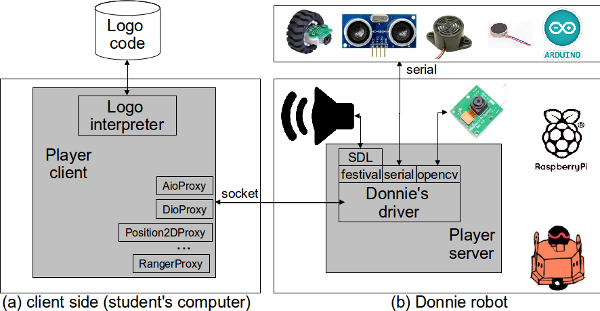
\includegraphics[width=0.95\linewidth]{figs/assistive-sw.png}
  \caption{Donnie's layered software stack.}
  \label{fig:donnie-soft-layer}
\end{figure}

As it is discussed later, novice students start coding with an ease to learn language for educational purposes (e.g. Logo). As this initial language starts to present limitations for the learning processes, it can be replaced for other languages with intuitive syntax (e.g. Ruby, Python), to finally move to more complex and complete languages such as C, C++, and Java. Currently, the Player robotic framework supports all languages mentioned before and it also has extensions to other more domain-specific languages such as Matlab \footnote{\url{http://playerstage.sourceforge.net/wiki/PlayerClientLibraries}} for numerical computing and Erlang \cite{Gruner:2009} for distributed systems. To the best of our knowledge, this is the first proposal of an educational language, similar to Logo, for Player. Moreover, thanks to the reuse of Player, this is the first assistive programming framework for robotics that supports so many languages.

In addition, the proposed system can also be used to teach multiple concepts of Computer Science, such as embedded programming, serial protocol, hardware/software interface, networked communication, topics of artificial intelligence (e.g. path finding, autonomous behavior), and computer vision (e.g. blob finder, tag recognition, pattern recognition), and advanced robotics (e.g. visual odometry, localization, mapping, multi-agent systems). Although at this stage of the project we are going to focus to teach programming to young students, the proposed system could also be used for high-school and graduate courses.

A crucial design decision was whether we would include a robotic software framework or not, and which framework to adopt. Current survey papers \cite{kramer2007,elkady2012} list dozens of robotic frameworks such as ROS, Orocos, Player, among others. The decision to support a framework was straight-forward since it enables to reuse useful codes (drivers and algorithms) to the proposed system. The second decision was which framework to adopt. Currently, ROS is probably the most used, documented, and with the biggest developer community \cite{quigley2009}. However, ROS is too complex for educational purposes, specially for students with little or none programming background. 

Player \cite{gerkey2003}, on the other hand, is much simpler in several aspects. First, it is based on a simpler client-server software design approach, compared to peer-to-peer, enabling simpler software design and hardware abstraction. The computational requirements to run Player is very low, which would fit nicely on an embedded processor. The source code is small (about 5 MBytes), the compilation process is straight-forward (few dependencies), there are several examples of robot drivers (there are dozen robots compatible with Player), and ready-to-use drivers for most common robotic resources (laser rangers, cameras, etc), it uses a simple textual configuration file to describe the robot drivers. Finally, Player/Stage are very active in the research community with currently more than 1500 citations just to the first paper \cite{gerkey2003}.

\subsubsection{Programming Languages}
\label{sec:prog-lang}

Choosing the initial programming language for young students with visual disabilities is an open problem. It has been reported that some languages are more difficult to students with visual disabilities. For example, Python uses whitespaces to delimit code blocks, which is hard to navigate with screen readers \cite{kane2014}. Languages such as C and Java use brackets to delimit code blocks, however, when the block is large with several sub-blocks, students with visual disabilities have difficult to find missing brackets.

The proposed system uses a Logo-based programming language because it was developed for educational context. Thus, the use of the Logo programming language is supported by a teaching methodology and an educational philosophy, which proposes the use of computers as a tool in the educational process~\cite{Valente1996}. To facilitate communication with the user, Logo commands are similar to natural language.

A new Logo-based language, called GoDonnie, is proposed to map the robot's capabilities. The complete specification of the language is presented in Table~\ref{tab:donnie-cmd}\footnote{GoDonnie language will be available in Portuguese and English.} and some examples of Portuguese commands are described below:


\begin{itemize}[topsep=0pt,itemsep=0ex,partopsep=0ex,parsep=0ex]
    \item Movement Commands:
    \begin{description}[topsep=0pt,itemsep=-1ex,partopsep=1ex,parsep=1ex]
        \item [PF:] It moves the robot forward for \textit{n} steps.
        \item [PT:] It moves the robot backwards for \textit{n} steps.
        \item [GD:] It spins the robot \textit{d} degrees to the right.
        \item [GE:] It spins the robot \textit{d} degrees to the left.
    \end{description}
    \item Selection Commands: 
    \begin{description}[topsep=0pt,itemsep=-1ex,partopsep=1ex,parsep=1ex]
        \item [SE:] It selects the code block to be executed based on the boolean value of a predicate.
    \end{description}
    \item Loop Commands: 
    \begin{description}[topsep=0pt,itemsep=-1ex,partopsep=1ex,parsep=1ex]
        \item [PARA:] It has three parts: variable initialization; loop condition;  increment the initialized variable. While the condition is true the robot executes the code block.
        \item [REPITA:] It repeats the code block \textit{t} times.
    \end{description}
    \item Position and Perception Commands:
    \begin{description}[topsep=0pt,itemsep=-1ex,partopsep=1ex,parsep=1ex]
        \item [CORES:] It returns the number of objects of a determined color \textit{c}.
        \item [ESPIAR:] It scans objects in $180^{o}$ in front of the robot. Then it returns the color, the distance, and the angle to the detected objects.
        \item [DISTÂNCIA:] The robot has six range sensors to measure the distance from obstacles. This command returns  the distance of the sensor \textit{r} to an object in steps.
        \item [ESTADO:] It returns series of current information about the robot such as its current pose, and the last instruction.
        \item [POS:] It returns the Cartesian \textit{X}, \textit{Y}, or angle \textit{A}.
    \end{description}
    \item Audio Commands:
    \begin{description}[topsep=0pt,itemsep=-1ex,partopsep=1ex,parsep=1ex]
        \item [SOM:] It turns on or off the robot sounds.
        \item [BIP:] It makes a noise in a chosen tone \textit{t} and period of time \textit{d}.
        \item [FALAR:] It speaks a phrase or word \textit{w} using a TTS.
    \end{description}
    \item Procedure Command:
    \begin{description}[topsep=0pt,itemsep=-1ex,partopsep=1ex,parsep=1ex]
        \item [APRENDER:] It implements procedures with an arbitrary number of arguments. This procedure can be called from any point of the program.
    \end{description}
\end{itemize}

More commands and usage information can be found in appendix A.

%\subsection{Assistive IDE}
%\label{sec:assit-ide}

%The developed IDE with textual interface is compatible with screen readers and magnification software. The IDE also has menus and shortcut keys to ease navigation; it narrates the debug log files, 

%\todo{INCLUIR FEATURES. Acredito que esta secao deva ser removida pois desenvolvemos muito pouco neste assunto.}

%\begin{figure}[h!]
%  \centering
%    
\includegraphics[width=0.5\textwidth]{figs/blank.jpg}
%  \caption{Assistive IDE screenshot.}
%  \label{fig:donnie-ide}
%\end{figure}

%%%%

\subsubsection{Graphical Simulation Environment}
\label{sec:simul}

The Player robotic framework is compatible with a lightweight 2D graphical simulation environment for multi robots called Stage \cite{Vaughan:2008}. This simulation environment is an option when the physical robots are not available. The main advantage is that the student`s software code does not change when the user migrates from virtual to physical robots or vice versa.
Stage simulates a population of multiple mobile robots, sensors and objects in a scene. It is designed to provide a computationally cheap and simple models of various devices, instead of trying to simulate devices with great fidelity. For this reason the Stage can simulate hundreds of robots in the same environment \cite{Vaughan:2008}, a feature that could be used for educational purposes, like in competition among the students where each student controls a robot and all robots share the same environment. 

The student can choose to use the simulated or the real robot, if this is available. We built Donnie's simulation models to be as close as possible to the real robot (Figure~\ref{fig:stage}(a)) such that the student can start debugging the software with simulation and use the real robot latter, when the code is more stable. Since Stage is graphical, we added sound to the robot's actions such that the students with visual disabilities can follow the steps of the robot. This feature is described in the next section.

The Figure~\ref{fig:stage}(b) shows a Stage screenshot, with one of the scenarios used for teaching that represents a room with one person, few tables, and sofas. A Stage scenario is described in a text file, with a simple syntax that enable students to create their own scenarios. The only non-textual part of a scenario definition is the description of the walls. This part requires drawing the walls with a software like Paintbrush, as illustrated in Figure~\ref{fig:stage}(c). %The students with visual disabilities receive also a floorplan of the scenario with Braille and tactile transcriptions of the environment (Figure~\ref{fig:stage}(c)). Then, the student is, for example, asked to find an object in the room. 


\begin{figure}[h!]
    \centering
    \begin{subfigure}[b]{0.7\linewidth}
        \centering
        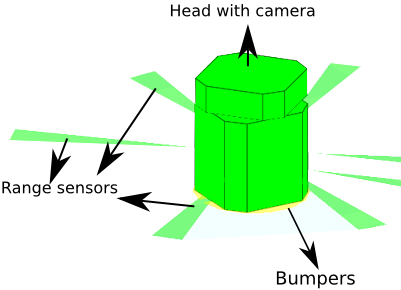
\includegraphics[width=\linewidth]{figs/donnie-simul.png}
        \caption{Donnie's virtual model.}
        \label{fig:donnie-simul}
    \end{subfigure}

    \begin{subfigure}[b]{0.7\linewidth}
        \centering
        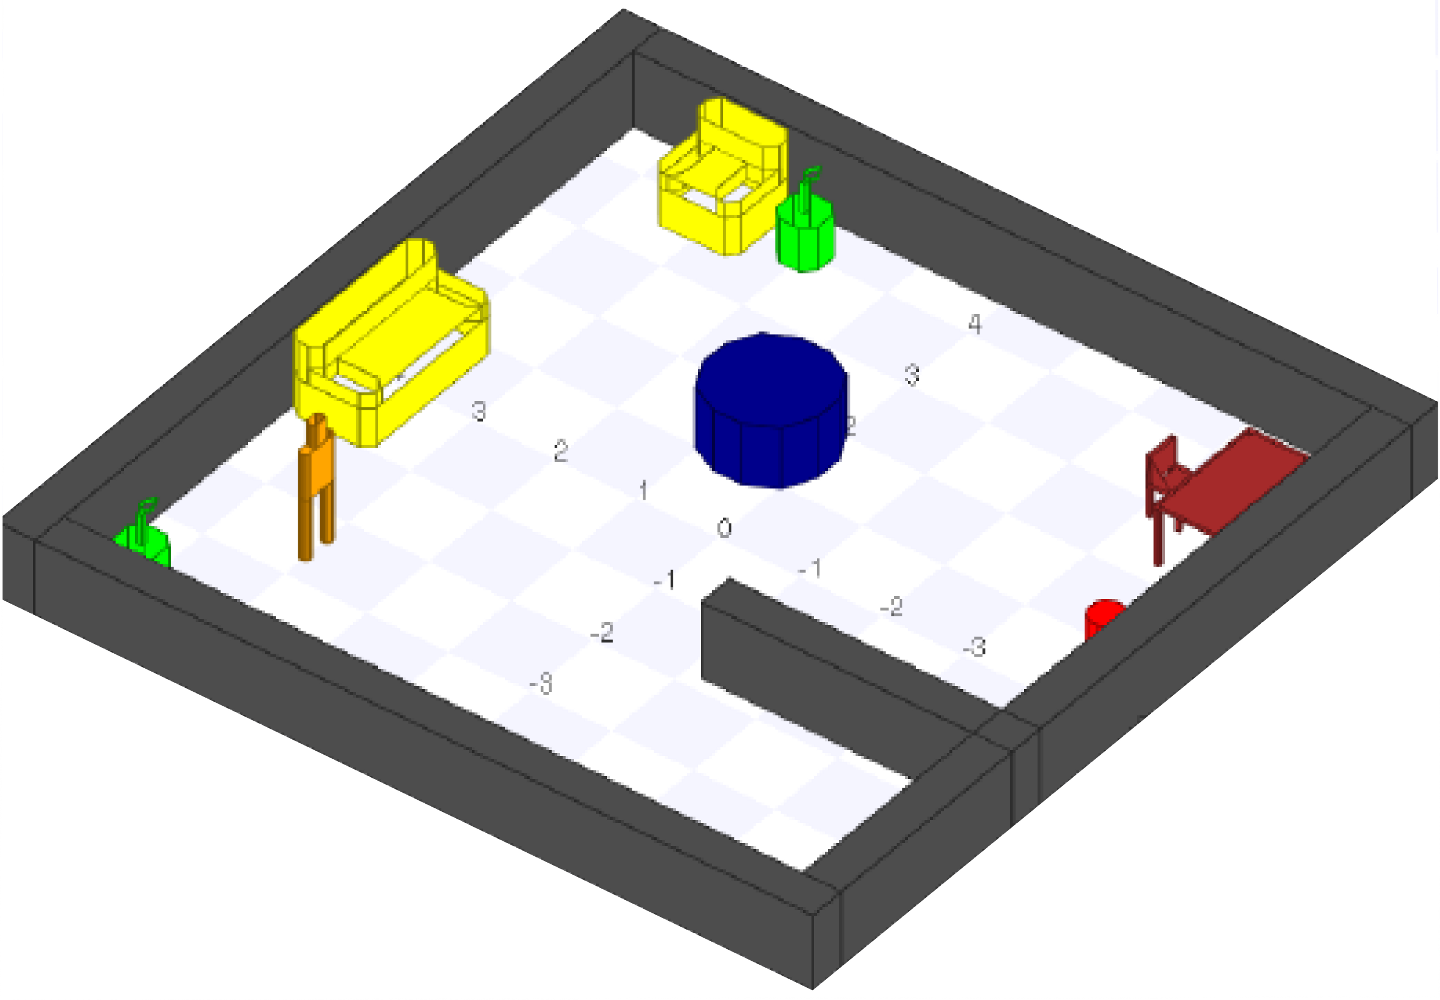
\includegraphics[width=\linewidth]{figs/stage-env.png}
        \caption{Screenshot of a Stage scenario.}
        \label{fig:stage-screen}
    \end{subfigure}

    %\begin{subfigure}[b]{0.47\linewidth}
    %    \centering
    %    
\includegraphics[width=\linewidth]{figs/blank.jpg}
    %    \caption{Braille and tactile description.}
    %    \label{fig:five over x}
    %\end{subfigure}
    
        \begin{subfigure}[b]{0.7\linewidth}
        \centering
        
\includegraphics[width=0.8\linewidth]{figs/mapa-stage.png}
        \caption{The png file for drawing the walls.}
        \label{fig:stage-wall}
    \end{subfigure}

    \caption{Stage-based virtual environment}
    \label{fig:stage}
\end{figure}


%%%%

\subsubsection{Donnie's Device Driver}
\label{sec:driver}

The Donnie's driver running on the RPi board is a Player driver~\cite{vaughan2007}, which connects the clients (student's computers) with the robot (either virtual or physical robot). It abstracts from the client software how the hardware resources are accessed. For example, the student can call a proxy interface called RangeProxy to read data from the sonar ring. It abstracts which low-level protocol is actually used, the brand of sensor, etc. Player has a set of predefined proxy interfaces~\cite{vaughan2007} for the most common robot resources like range sensors, cameras, grippers, motors, position, map, among dozens of other interfaces available. 

A Player driver is a piece of software used to remotely access the robot using these proxy interfaces. Donnie's Player driver uses the following set of existing interfaces:

\begin{itemize}
\item Position2d: used both to move and to get the robot's position;
\item Ranger: used to access the ring of seven ultrasonic sensors;
\item Blobfinder: returns a list of blobs capture in the image frames;
\item Dio (Digital IO): interface to read and write binary devices such as LEDs, buzzer, vibration motors;
\item Power: interface used to read battery status;
\item Bumper: detects collision from the bumper sensors;
\item Aio (Analog IO): interface to read and write analog devices such as light intensity sensor.
\end{itemize}

The following set of interfaces are under development:

\begin{itemize}
\item Speech: performs text synthesis with Festival text-to-speech \cite{black2001} and Google TTS;
\item Audio: plays various audio formats with the Sound eXchange (SoX) library \footnote{\url{http://sox.sourceforge.net/libsox.html}};
\item PiCamPlayer: A new Player driver to grab image frames from the RaspiCam;
\item BlobFinder: An updated Player driver, based on OpenCV 3.0, to detect blobs from cameras.
\end{itemize}

%\todo{Amory: A lista esta completa só nao tem o proxy speech e nem o proxy audio. O proxy AIO serviria para ler um sensor diverso tipo LDR ou um sensor de intensidade campo magnetico (Efeito Hall) mas não estamos usando isso no momento então eu tirei. Também não temos um proxy para line follower entao seria usado o DIO para isso.}

As illustrated in Figure~\ref{fig:donnie-soft-layer}, the requests to the interfaces position2d, ranger, among others are actually implemented in the Arduino board. Thus, the Player driver only translates the serial protocol to/from remote wifi access using Player`s built-in methods. On the other hand, the request to camera, blobfinder, and sound interfaces are actually executed in the RPi board. 
%The camera-related interfaces uses OpenCV for image processing while the sound-related interface uses Simple DirectMedia Layer (SDL) \footnote{\url{www.libsdl.org}} to play .wav files and Festival text-to-speech \cite{black2001}.

\begin{lstlisting}[language=C,frame=lines,xleftmargin=5.0ex, caption={Player-based device driver.},label=lst:donnie-driver]  
arduino = Serial(cfg_serial_port)
// main loop
while(TRUE) {
    processIncomingData()
    ProcessMessages()
    usleep(10)
}
\end{lstlisting}


Listing~\ref{lst:donnie-driver} presents a simplified view of the driver structure. It`s main goal is to translate clients requests. It initially sets up the serial port (line 1). Then, in an infinite loop, it treats incoming data from the Arduino (line 4) as, for example, tick count from the wheels, and it treats the incoming client`s requests (line 5) as, updated range data. Each of these two main functions is just a big switch case for every message type coming from the Arduino or the client computer, respectively.

The device driver is also responsible for generating sound clues that enables the student to follow the robot's movement. 
There are three types of sounds that Donnie can issue: movement sounds, stall sounds, and voice feedback. When Donnie moves, both the simulation model and the physical robot, it makes a sound that features it's movement. For example, one sound for moving forward, other for moving backward, and turning left/right. The stall sound works in a similar way, giving a feedback for the user when the robot hits or detects a wall with its bumpers and range sensors. Donnie can also give a voice feedback to the user when certain commands are executed, like the status commands. All types of sounds and the spoken language can be selected in a readable textual configuration file. Festival TTS currently supports English or Spanish while Google TTS supports several languages, including Brazilian Portuguese. However, Google TTS can only be used when the robot has Internet connection.

%%%%

\subsubsection{Donnie's Arduino Firmware}
\label{sec:firm}

Listing~\ref{lst:donnie-firm} presents a simplified view of the firmware structure running on the Arduino board. The main initial loop (line 1 to 5) waits for an initial configuration packet sent from the Player driver to the Arduino via the serial port. The robot does not start until this configuration packet is received, however, the power status is checked to alert the battery status. The firmware has series of configurable parameters detailed below: 

\begin{itemize}
\item PID parameters;
\item individual sensor update frequencies;
\item battery status parameters;
\item configurable pin ports.
\end{itemize}

%\todo{amory: esses sao os parametros que estamos usando by marques}

\begin{lstlisting}[language=C,frame=lines,xleftmargin=5.0ex, caption={Arduino-based firmaware.},label=lst:donnie-firm]  
do{
  sendRequestConfig() //request a robot config from driver
  cmd = readCommand() //receive robot config
  power_update() //check battery status
}while(cmd != CONFIGPACK) // wait until robot config received

// main loop
while(TRUE) {
  cmd = readCommand()  //Read incoming command from serial port
  processCommand(cmd)  //Execute requested command
  updateSensors()  //Read each sensor and update variables
  updateIndicators()  //Update leds, vibs and buzzer indicators
  sendData() //Send data to serial port
  updateTicks()  //Increment the tickCnt each 1ms (1000us)
}
\end{lstlisting}


The main loop in Listing~\ref{lst:donnie-firm} (lines 8 to 15) performs the robot control. It initially reads incoming packets from the serial port (line 9), it executes the commands (line 10) (e.g. move commands), it updates the sensor readings (line 11) into the internal memory, it updates the indicators (LEDs, buzzer, vibration motors) based on the command and sensor readings (line 12), and it sends the new data (line 13) via serial port to the Player Driver. 

%processCommand(cmd) {  
%	SWITCH(cmd){
%		CASE PINGPACK:
%			...
%		CASE DIOPACK:
%			...
%		CASE MOTORPACK:
%			...
%	}
%}
%
%void updateSensors(){
%	IF(tickCnt % UPDATE_DIO_FRQ == 0){
%		...
%	}
%	IF(tickCnt % UPDATE_RANGER_FRQ == 0){
%		ranger_update();
%	}
%	IF(tickCnt % 200 == 0){
%		power_update(tickCnt);
%	}
%	bumper_update();
%}
%
%
%sendData(){
%
%	IF(tickCnt % SEND_DIO_FRQ == 0){
%		sendSystemDioMsg(systemDio_data,5);
%	}
%	IF(tickCnt % SEND_RANGER_FRQ == 0){
%		sendRangerMsg(range,6);
%	}
%	IF(tickCnt % SEND_BUMPER_FRQ == 0){
%		sendBumperMsg(bumper,6);
%	}
%	IF(tickCnt % SEND_POWER_FRQ == 0){
%		sendPowerMsg(power);
%	}
%	IF(tickCnt % SEND_PING_FRQ == 0){
%		sendPing();
%	}
%}
%
%sendPowerMsg(data){
%    tx_data[0]=POWERPACK
%    tx_data[1]=lowBytes(data)
%    tx_data[2]=HighBytes(data)
%    tx_data_count = 3
%    writeData(tx_data,tx_data_count)
%}
%

%%%%

\subsubsection{Serial Communication Protocol}
\label{sec:serial}


The interface between RPi and Arduino is via a serial port. This section describes its protocol, illustrated in Figure~\ref{fig:serial-format}. The serial communication is another software layer which could be explored for teaching the concepts of data transfer, latency, bandwidth, data serialization, the memory sizes of scalar types, binary data representation, and finite state machine for building the protocol.

The protocol format presented in Figure~\ref{fig:serial-format} has two constants bytes of header, one byte of packet length, one byte for message types, variable number of bytes for the payload, and a final byte with checksum. Each functionality in the Arduino board has a corresponding message type. The most relevant message types are presented in Table~\ref{tab:serial-protocol}.

\begin{figure}[h!]
  \centering
    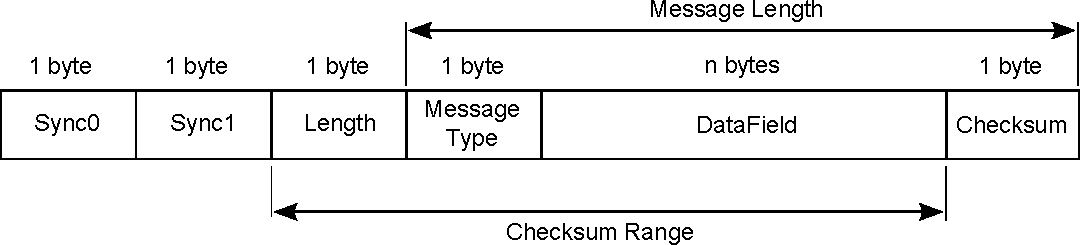
\includegraphics[width=0.45\textwidth]{figs/protocol.pdf}
  \caption{Serial packet format.}
  \label{fig:serial-format}
\end{figure}


\begin{table}[h]
  \caption{A sample of Donnie's serial communication protocol.}
  \label{tab:serial-protocol}
\begin{center}
  \begin{tabular}{ p{1.6cm} | p{3cm} | p{2.6cm} }
    \bf{message name} & \bf{description} & \bf{fields}\\
    \hline
    MOTORSTATE & defines direction and velocity for both motors & direction (left/right/on/off); right motor speed; left motor speed   \\
    \hline
    HEAD & defines the angular position of robot's head & mode (SCAN/SETPOS/GOTO); servo angle\\
    \hline
    RANGER & defines the 6 ultrasonic data & number of sensors; sensors data received \\
    \hline
    BUMPER & defines the 4 bumper data & number of sensors; sensors data received \\
    \hline
    POWER & defines the current battery voltage & float number indicating the measured voltage \\
    \hline
    ENCODER & defines wheel ticks from the wheel encoders & right wheel ticks; left wheel ticks \\
    \hline
    CONFIG & configures the micro-controller parameters using the parameters from a config file & any parameter defined in the config file (.cfg) \\
    \hline
    REQ\_CONFIG & requests from micro-controller for the parameters in the configuration file & none \\
    \hline
    REQ\_PING & requests from micro-controller to check the serial connection status & none \\
    \hline
    PING & used to check the serial connection status & none \\
    \hline
  \end{tabular}
\end{center}
\end{table}

When the student adds a new functionality to the robot, he/she has to define a new message type and adapt both the firmware and the driver to handle this new message.
The firmware and driver codes have comments to give clues to the students to find where to change.
